\section{Sequence, List}
\label{sec:Sequence}
%%%%%%%%%%%%%%%%%%%%%%%%%%%%%%%%%%%%%%%%%%%%%%%%%%%%%%%%
\begin{figure}[h!]
\begin{center}
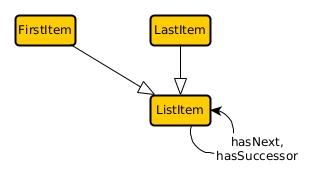
\includegraphics[width=.8\textwidth]{figures/sequence}
\end{center}
\caption{Schema Diagram for the Sequence and List Pattern. The visual notation is explained in Chapter \ref{chap:prelims}.}
\label{fig:Spatiotemporal}
\label{fig:Sequence,}
\end{figure}
\subsection{Summary}
\label{sum:Sequence}
%%%%%%%%%%%%%%%%%%%%%%%%%%%%
The \textsf{Sequence} Pattern is a way of imposing order upon items of interest; it follows the conceptualization of a Linked List from computer science. This pattern is a simplified view of the \textsf{Tree} Pattern (as found in Section \ref{sec:Tree}) and is adapted from \cite{tree}. While this pattern seems very abstract, it is both easy to specialize and occurs very frequently. In this resource, the pattern occurs in the \textsf{Trajectory} Pattern (a sequence of Fixes), the \textsf{SpatiotemporalExtent} Pattern (a sequence of \textsf{Place}, \textsf{Time} pairs), and \textsf{SpatialExtent} (a sequence of \textsf{PointsInSpace}.

%%%%%%%%%%%%%%%%%%%%%%%%%%%%%%%%%%%%%%%%%%%%%%%%%%%%%%%%
\subsection{Axiomatization}
\label{axs:Sequence,}
%%%%%%%%%%%%%%%%%%%%%%%%%%%%
\begin{align}
\textsf{FirstItem} &\sqsubseteq \textsf{ListItem} \\
\textsf{LastItem} &\sqsubseteq \textsf{ListItem} \\
\textsf{ListItem} &\sqsubseteq \forall \textsf{hasNext.ListItem} \\
\textsf{ListItem} &\sqsubseteq \forall \textsf{hasNext}^-\textsf{.ListItem} \\
\textsf{ListItem} \sqcap \lnot \textsf{LastItem} &\equiv \textsf{ListItem} \sqcap \mathord{=1}\textsf{hasNext.ListItem} \\
\textsf{ListItem} \sqcap \lnot \textsf{FirstItem} &\equiv \textsf{ListItem} \sqcap \mathord{=1}\textsf{hasNext}^- \textsf{.ListItem} \\
\textsf{FirstItem} &\equiv \textsf{ListItem} \sqcap \lnot \exists \textsf{hasNext}^-\textsf{.}\top \\
\textsf{LastItem} &\equiv \textsf{ListItem} \sqcap \lnot \exists \textsf{hasNext.}\top \\
\textsf{hasNext} &\sqsubseteq \textsf{hasSuccessor} \\
\textsf{hasNext} \circ \textsf{hasSuccessor} &\sqsubseteq \textsf{hasSuccessor} \\
\text{Irreflexive}&(\textsf{hasSuccessor})
\end{align}

%%%%%%%%%%%%%%%%%%%%%%%%%%%%%%%%%%%%%%%%%%%%%%%%%%%%%%%%
\subsection{Explanations}
\label{exp:Sequence}
%%%%%%%%%%%%%%%%%%%%%%%%%%%%
\begin{enumerate}
\item Subclass: the \textsf{FirstItem} is a \textsf{ListItem}.
\item Subclass: the \textsf{LastItem} is a \textsf{ListItem}.
\item Scoped Range: the range of \textsf{hasNext}, scoped by \textsf{ListItem}, is \textsf{ListItem}.
\item Scoped Range: the range of \textsf{hasNext}$^-$, scoped by \textsf{ListItem}, is \textsf{ListItem}.
\item A \textsf{ListItem} that is not the \textsf{LastItem} has exactly one next \textsf{ListItem}.
\item A \textsf{ListItem} that is not the \textsf{FirstItem} has exactly one previous \textsf{ListItem}.
\item The \textsf{FirstItem} does not have have a predecessor.
\item The \textsf{LastItem} does not have a next \textsf{ListItem}.
\item Subproperty: \textsf{hasNext} is a subproperty to \textsf{hasSuccessor}.
\item Role Chain: the successor of a \textsf{ListItem}'s next \textsf{ListItem} is its successor.
\item Irreflexivity.
\end{enumerate}

%%%%%%%%%%%%%%%%%%%%%%%%%%%%%%%%%%%%%%%%%%%%%%%%%%%%%%%%
\subsection{Competency Questions}
\label{cqs:Sequence}
%%%%%%%%%%%%%%%%%%%%%%%%%%%%
\begin{enumerate}[CQ1.]
\item What is the first element of the list?
\item What is the last element of the list?
\item Is $x$ a predecessor of $y$?
\end{enumerate}

\newpage
%%%%%%%%%%%%%%%%%%%%%%%%%%%%%%%%%%%%%%%%%%%%%%%%%%%%%%%%
% End Section
%%%%%%%%%%%%%%%%%%%%%%%%%%%%%%%%%%%%%%%%%%%%%%%%%%%%%%%%
%%%%%%%%%%%%%%%%%%%%%%%%%%%%%%%%%%%%%%%%%%%%%%%%%%%%%%%%